\chapter{Cuda Overview}\label{sec:cuda}
Cuda is a software layer that allow programmers to exploit the capability of Nvidia GPUs as general purpose processors.\\
Dealing with a video card in this way requires approaching a completely new programming style and acquiring some knowledge about the basic Nvidia GPUs architectures, even though all the internal details are masked by the framework.\\
%First of all, as a philosophical remark, a GPU cannot run anything conceived and written for a CPU, as every vector stream architecture. In order to product software that can be executed on a Cuda Capable GPU, the programmer must write natively parallel code using one of the supported languages, extended with ad hoc Cuda primitives. There is no tool that can perform automatic porting of a sequential code into a parallel one.\\
One of the most important feature of this framework is that it abstracts away all the physical details of the supported GPUs and exposes to the programmer always the very same logical organization, shown in Figure 3.1. These GPUs can be considered MIMD array of SIMD processors called MultiProcessors. Each MultiProcessor is mainly composed by 3 logic elements: a fixed number of cores, an instruction unit and a private memory space. Due to the property of abstraction mentioned before, the only difference between families of Nvidia products is in the number of MultiProcessor and in the dimensioning of the respective composing elements.\\

\begin{figure}[h!bt]
	\centerline{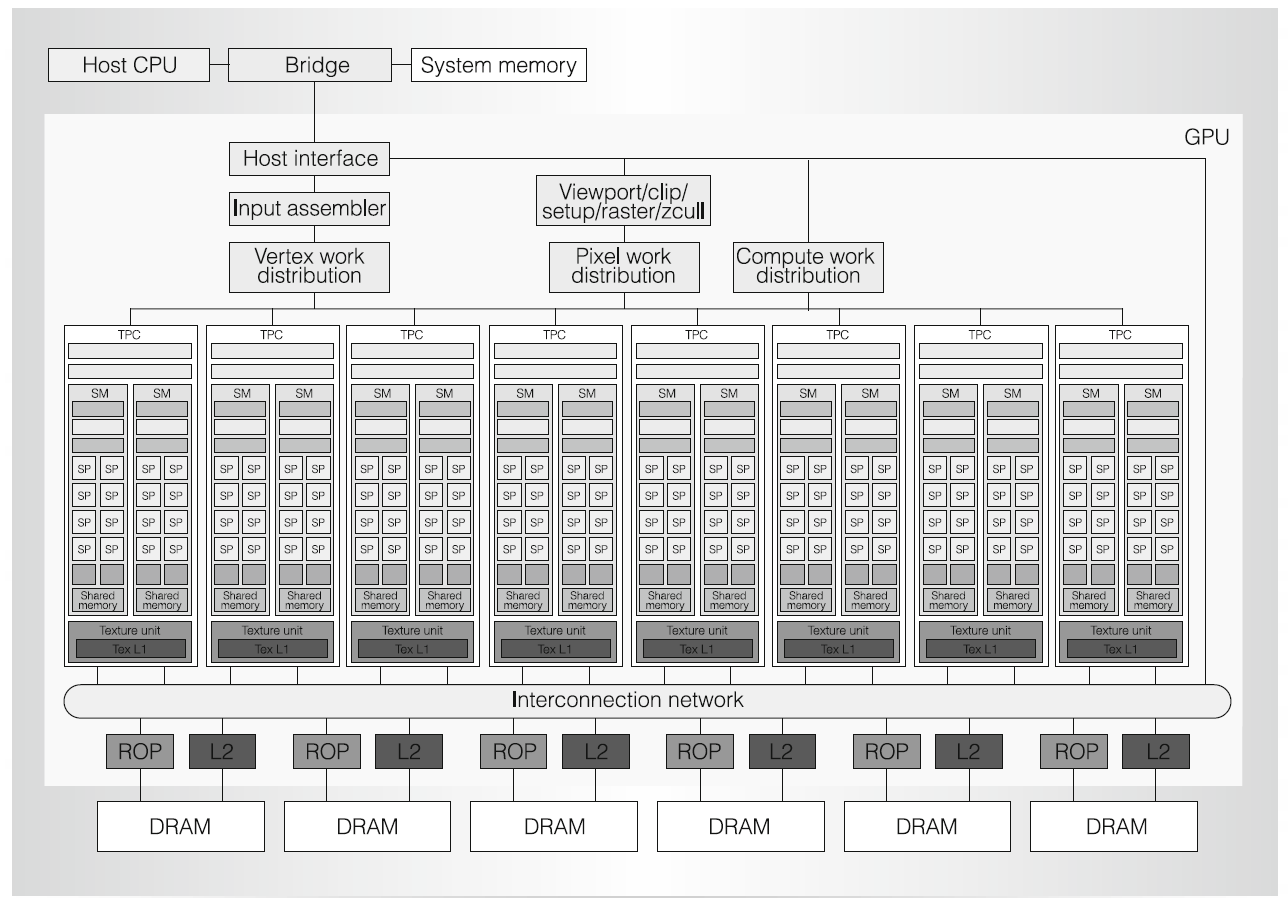
\includegraphics[width=\textwidth]{img/NvidiaGPUsLogicalOrg.png}}
	\caption{Logical Organization of all the Cuda capable devices. The programmer does not have to take care of the physical organization of the GPU that will actually execute the program.}
	\label{fig:NvidiaGPUsLogicalOrg}
\end{figure}

Cores Description: Simple and fast, high throughput (FP) and no speculation, double precision question, others...\\

Memory Hierarchy: OnChip --> Constant/Texture Cache, Registers; Off-Chip --> Global, Constant, Texture.\\
Mem Img. \\

Programming Model: Thread, Block, Grid, Sync.\\

Best Practices: Memory Accesses, Sync, others.\\
